\documentclass{article}
%documentclass[draft]{article}

\usepackage[italian]{babel}
\usepackage[utf8]{inputenc}


\usepackage{graphicx} % Immagini fantastiche e...
\graphicspath{        % dove trovarle
  {./images/},
}

%%% Bibliografia
%\usepackage{csquotes}
%\usepackage{biblatex}
%\addbibresource{bibl.bib}


% Grafici direttamente in latex
\usepackage{tikz}
\usetikzlibrary{shapes,positioning,calc}
\colorlet{lightgray}{gray!20}

\usepackage{rotating} % per tabella ruotata
\usepackage{makecell}
%\usepackage[showframe=true]{geometry}
\usepackage{changepage}

% Immagini galleggiano
\usepackage{float}

\usepackage{color}

\usepackage{caption}
% per caption ad immagini in tab annidiate
\usepackage{subcaption}

\usepackage{hyperref} % lasciare per ultimo
%\hypersetup{colorlinks=true, linkcolor=blue, citecolor=black, plainpages=false, urlcolor=blue}
\hypersetup{colorlinks=true, linkcolor=black, citecolor=black, plainpages=false, urlcolor=blue}

% Usato nella copertina
\usepackage{wallpaper}



\usepackage{listings}
\lstset{
  showspaces=false,
  showstringspaces=false,
  basicstyle=\footnotesize,
  %basicstyle=\tiny,
  %basicstyle=\ttfamily,
  %numbers=left,
  %numbers=none,
  numberstyle=\small,
  mathescape
}

\usepackage{algpseudocode,algorithm,algorithmicx}


% Simboli matematici
%\usepackage{amsthm}
\usepackage{amssymb}
\usepackage{amsmath}
%\usepackage{amsfonts}
%\usepackage{mathabx} % per \topdoteq
%\usepackage{mathtools, amsthm}


% Comodo per evidenziare zone da modificare
\usepackage{todonotes} 

% Lorem ipsum...
\usepackage{lipsum} 


 
% ================================ %
%          Cose Personali          %
% ================================ %

% Alcune comodita' logico/matematiche
\let\ep\epsilon
\let\b\bullet
\let\iff\Leftrightarrow
\newcommand{\viff}{\Updownarrow}
\let\impl\Rightarrow

\newcommand{\norm}[1]{\lvert\lvert #1 \lvert\lvert}
\newcommand{\Norm}[1]{\Big\lvert \Big\lvert #1 \Big\lvert \Big\lvert}

\newcommand\N{\ensuremath{\mathbb{N}}}
\newcommand\R{\ensuremath{\mathbb{R}}}
\newcommand\Z{\ensuremath{\mathbb{Z}}}
\renewcommand\O{\ensuremath{\emptyset}}
\newcommand\Q{\ensuremath{\mathbb{Q}}}
\newcommand\C{\ensuremath{\mathbb{C}}}

\newcommand\E{\ensuremath{\mathbb{E}}}
\newcommand\T{\ensuremath{\mathbb{T}}}
\renewcommand\inf{\ensuremath{\infty}}




% ================================ %
%            Il Documento          %
% ================================ %
\begin{document}

% ================================ %
%        Creo Prima Pagina         %
% ================================ %

\ThisCenterWallPaper{0.95}{polloPallido}
% Intestazione
% TODO Migliorare esteticamente
\begin{titlepage}
 	\centering
  \Huge{\textbf{Progetto Ragionamento Automatico}}\\
 	[30mm]
 	\centering
  \Huge{\textbf{Studente: Tristano Munini}}\\
 	%[25mm]
  %\raggedright
  %\Large{\textbf{Corso:}}\\
  %\Large{\textbf{TODO}}\\
 	[125mm]
 	\centering
  \LARGE{\underline{\textbf{ANNO ACCADEMICO 2019-2020}}}\\
\end{titlepage}

%% ================================ %
%%              Indice              %
%% ================================ %
%\tableofcontents
%\thispagestyle{empty}
%\cleardoublepage
%\setcounter{page}{1}


% ================================ %
%      Qua Inizia La Tesina        %
% ================================ %
%\abstract{
%  \lipsum[1]
%}

%\pagenumbering{gobble} % TODO REMOVE


%!TEX TS-program = pdflatex
%!TEX root = main.tex
%!TEX encoding = UTF-8 Unicode

\section{Il problema}
Si riporta il testo della consegna
\begin{figure}[ht]
  \centering
  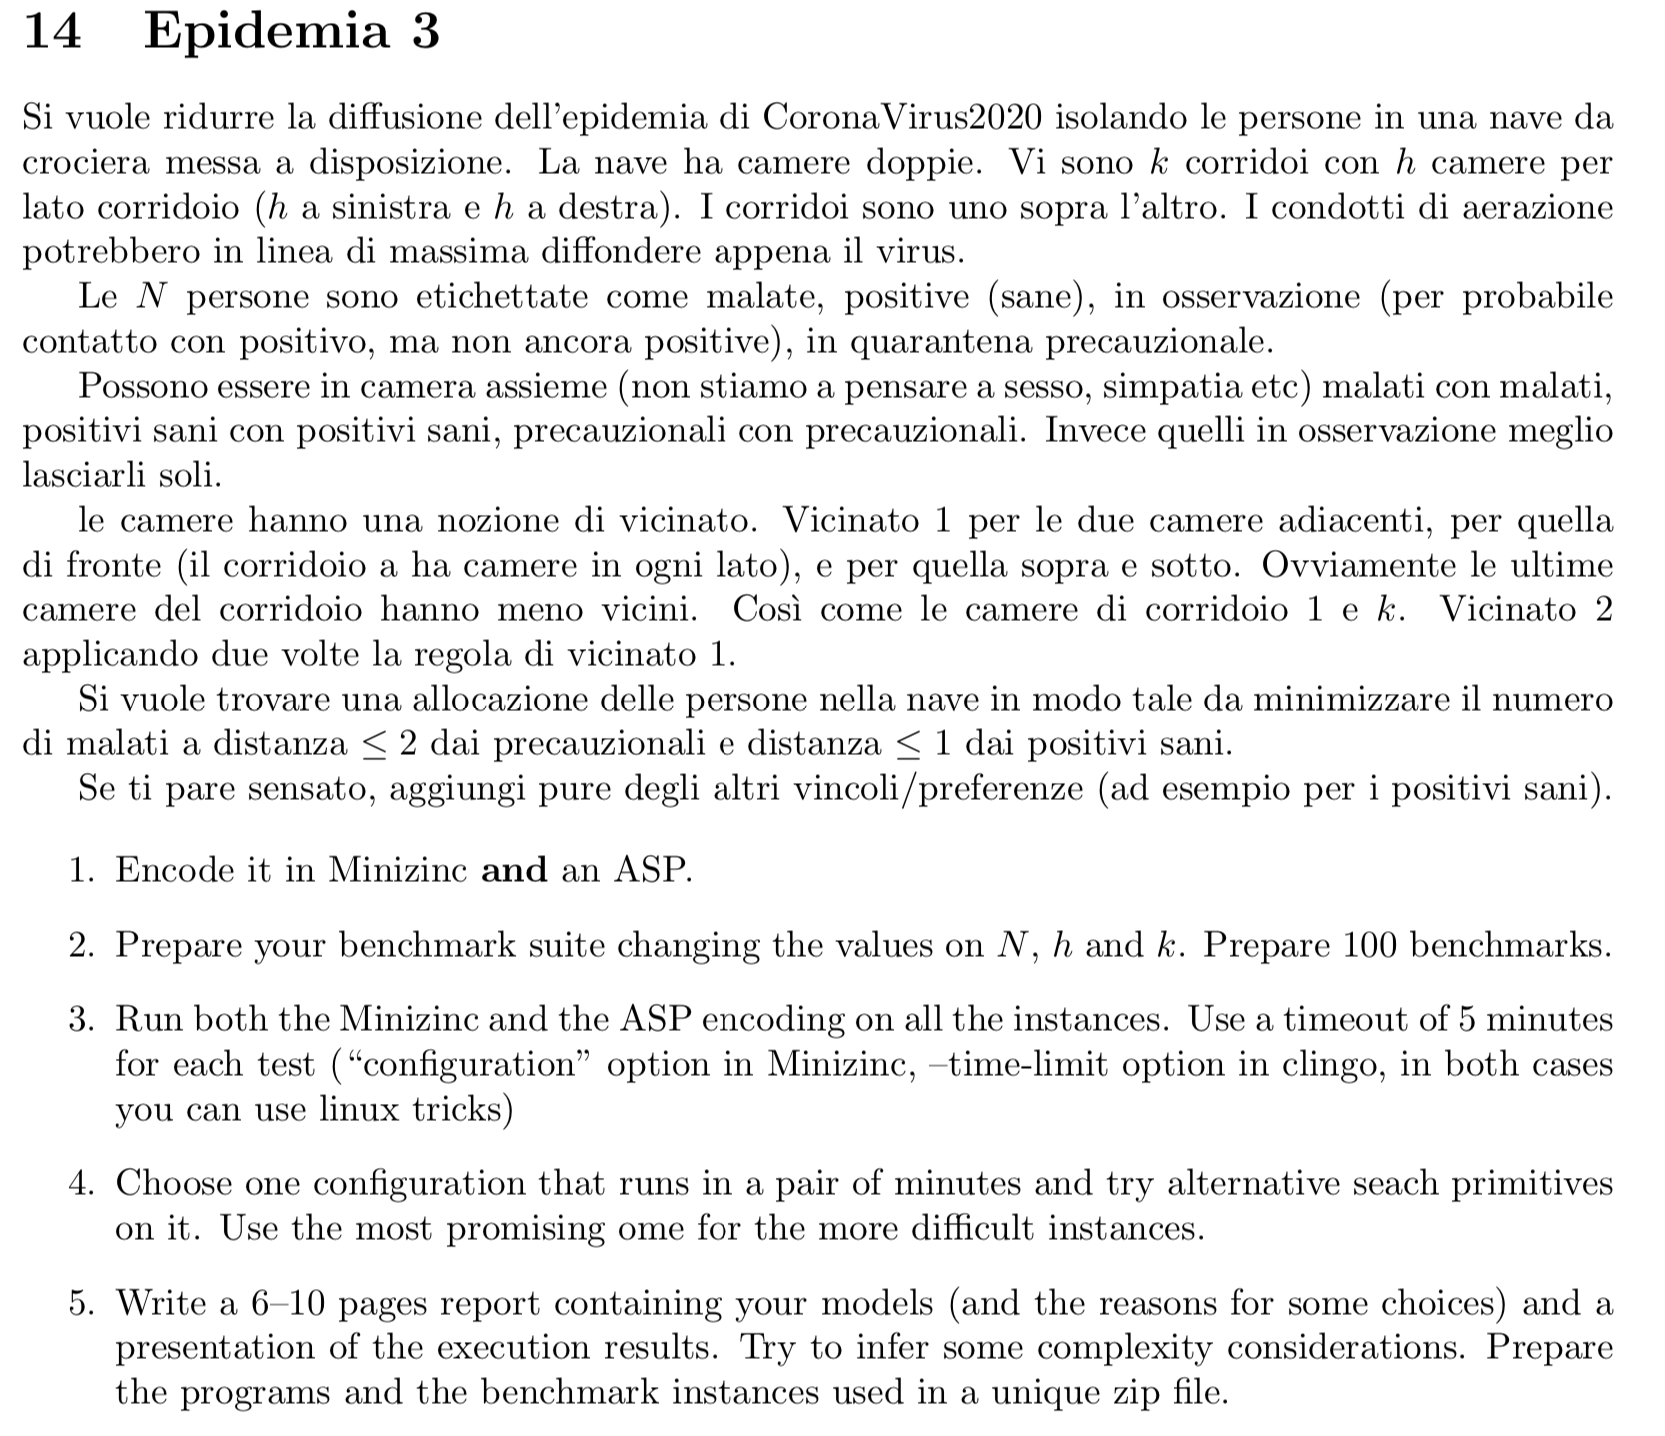
\includegraphics[width=\textwidth]{MUNINI}
\end{figure}

%!TEX TS-program = pdflatex
%!TEX root = main.tex
%!TEX encoding = UTF-8 Unicode

\section{ASP}
\subsection{Il modello}
%In input vengono forniti
%\lstinline{K, H, M, O, P, Q}

Ad ogni stanza viene associato un intero partendo da 0 ed incrementando di 1.
Il numero totale di stanze è $2*K*H$, perché abbiamo $K$ corridoi e per ciascun corridoio ci sono $H$ stanze per lato (sinistro o destro).
Con questa numerazione ogni $K$ numeri si cambierà lato, mentre ogni $2*K$ numeri si indica un corridoio ad un piano superiore.
La numerazione permette di modellare abbastanza facilmente le relazioni spaziali tra stanze,
ad esempio:
le prime $H$ stanze appartengono al lato destro del primo corridoio;
le stanze dalla $H$ alla $2*H-1$ appartengono al lato sinistro del primo corridoio;
le stanze dalla $2*H$ alla $3*H-1$ sono sul secondo piano a destra; etc\dots

\noindent
Nel file \emph{covid19.lp} le stanze vengono definite con
\lstinputlisting[firstline= 7, lastline = 7]{./code/covid19.lp}

\noindent
Poiché gli ospiti devono essere assegnati esattamente ad una stanza, si definiscono i vincoli
\lstinputlisting[
firstline= 10,
lastline = 13
]{./code/covid19.lp}

\noindent
Poiché le stanze hanno capacità limitate, che dipendono dal tipo di ospite, risulta necessario definire
\lstinputlisting[
firstline= 16,
lastline = 22
]{./code/covid19.lp}

\noindent
Inoltre una stanza può essere condivisa solo da ospiti dello stesso tipo (esclusi i positivi),
quindi vengono vietate tutte le coppie illecite
\lstinputlisting[
firstline= 25,
lastline = 32
]{./code/covid19.lp}

\noindent
Due camere sono a distanza \emph{Vicinato 1} se rispettano uno dei vincoli tra
\lstinputlisting[
firstline= 36,
lastline = 62
]{./code/covid19.lp}
\todo{spiegare la matematica?}

\noindent
Due camere sono a distanza \emph{Vicinato 2} se condividono una camera a distanza \emph{Vicinato 1}.
In pratica, presa una camera, un elemento nel suo \emph{Vicinato 2} può essere raggiunto in due passi selezionando prima un \emph{Vicinato 1} adeguato e poi un \emph{Vicinato 1} della camera appena selezionata.
Nel vincolo si richiede l'esistenza di questa terza camera che faccia da ``perno'' per lo spostamento.
\lstinputlisting[
firstline= 65,
lastline = 68
]{./code/covid19.lp}

\noindent
La funzione da minimizzare viene calcolata contando che ospiti di che stanze soddisfano la relazione \emph{scomodo}.
Due ospiti non possono soddisfare la relazione se occupano stanze non in vicinato tra loro, oppure se appartengono a tipologie non problematiche (es. in osservazione).
\lstinputlisting[
firstline= 99,
lastline = 106
]{./code/covid19.lp}
\todo{allungare?}

%\cleardoublepage
\subsection{\emph{Symmetry Breaking}}
Poiché non ci sono differenze tra malati dello stesso tipo è possible fissare un ordinamento arbitrario.
In questo caso ad ospiti con un indice inferiore vengono assegnate camera ai piani più bassi.
\lstinputlisting[
firstline= 75,
lastline = 78
]{./code/covid19.lp}

\noindent
Osservando che le camere all'inizio ed alla fine dei corridoi hanno un numero inferiore di camere in \emph{Vicinato 1} (e quindi anche in \emph{Vicinato 2}), risulta sensato fissare il primo malato nella prima stanza disponibile, ossia nella prima stanza del primo corridoio.
\todo{giustificare meglio?}
\lstinputlisting[ 
firstline= 73,
lastline = 73
]{./code/covid19.lp}

%!TEX TS-program = pdflatex
%!TEX root = main.tex
%!TEX encoding = UTF-8 Unicode

\section{Minizinc}
\subsection{Il modello}
%In input vengono forniti
%\lstinline{K, H, M, O, P, Q}
Ad ogni stanza viene associato un intero partendo da 0 ed incrementando di 1.
Il numero totale di stanze è $2*K*H$, perché abbiamo $K$ corridoi e per ciascun corridoio ci sono $H$ stanze per lato (sinistro o destro).
Con questa numerazione ogni $K$ numeri si cambierà lato, mentre ogni $2*K$ numeri si indica un corridoio ad un piano superiore.
La numerazione permette di modellare abbastanza facilmente le relazioni spaziali tra stanze,
ad esempio:
le prime $H$ stanze appartengono al lato sinistro del primo corridoio;
le stanze dalla $H$ alla $2*H-1$ appartengono al lato destro del primo corridoio;
le stanze dalla $2*H$ alla $3*H-1$ sono sul secondo piano a sinistra; etc\dots
\lstinputlisting[
firstline= 1,
lastline = 16
]{./code/covid19.mzn}

\noindent
Le limitazioni sul numero di ospiti per stanza sono date dai seguenti vincoli.
Notare come questa modellazione permette di usare \emph{alldifferent} sui numeri stanze degli ospiti in osservazione.
\lstinputlisting[
firstline= 19,
lastline = 50
]{./code/covid19.mzn}

\noindent
La relazione di \emph{Vicinato 1} verifica se due stanze sono adiacenti per una delle cinque direzioni (sopra, sotto, destra, sinistra e di fronte).
\lstinputlisting[
firstline= 53,
lastline = 77
]{./code/covid19.mzn}

\noindent
Due camere sono a distanza \emph{Vicinato 2} se condividono una camera a distanza \emph{Vicinato 1}.
In pratica, presa una camera, un elemento nel suo \emph{Vicinato 2} può essere raggiunto in due passi selezionando prima un \emph{Vicinato 1} adeguato e poi un \emph{Vicinato 1} della camera appena selezionata.
Nel vincolo si richiede l'esistenza di questa terza camera che faccia da ``perno'' per lo spostamento.
%\emph{Vicinato 2} viene soddisfatto se esiste una terza stanza su cui fare ``perno'' in \emph{Vicinato 1} con entrambe le stanze considerate
\lstinputlisting[
firstline= 80,
lastline = 87
]{./code/covid19.mzn}

\noindent
%%Il valore da minimizzare è calcolato allo stesso modo del codice ASP
%La funzione da minimizzare viene calcolata contando che ospiti di che stanze soddisfano la relazione \emph{scomodo}.
%Due ospiti non possono soddisfare la relazione se occupano stanze non in vicinato tra loro, oppure se appartengono a tipologie non problematiche (es. in osservazione).
Si vuole minimizzare un intero $c$ calcolato contando tutte le coppie di ospiti con tipologia scomoda (malato, quarantena precauzionale, positivo) in \emph{Vicinato 1} oppure \emph{Vicinato 2}, a seconda della tipologia.
%In particolare si vuole che i malati non siano i
Notare che $c$ ha un valore più grande se nelle stanze in vicinato ci sono più ospiti, come si vede in \autoref{fig:esempio_1}, in cui $c=4$ a causa dei malati nella stanza $1$ in \emph{Vicinato 2} con gli ospiti in quarantena della stanza $7$.
Le stanze si contano partendo da quella in alto a sinistra, stanza numero 0 e prima stanza a sinistra del primo corridoio, e procedendo per righe.
Ogni due righe si sale al corridoio superiore, come indicato dai numeri sulla destra.
\lstinputlisting[
firstline= 90,
lastline = 99
]{./code/covid19.mzn}
\begin{figure}[ht]
  \centering
  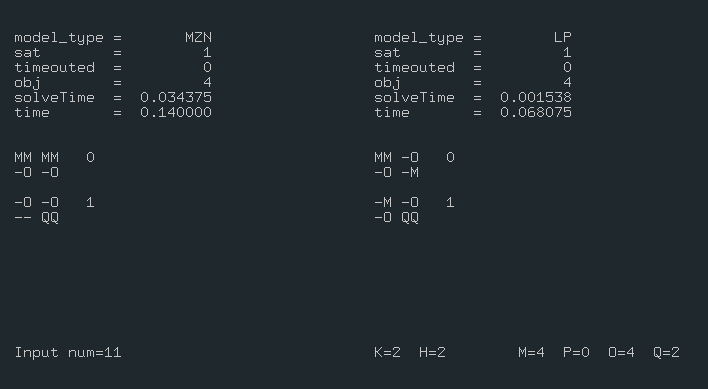
\includegraphics[width=.8\textwidth]{esempio_1}
  \caption{Schermata di \emph{in\_out\_visualizer.py}}
  \label{fig:esempio_1}
\end{figure}

\noindent
La configurazione che ha dato i risultati migliori è riportata nel listato che segue.
Notare come si tenti fin da subito di raccogliere ospiti malati o in osservazione nelle prime stanze e sui piani più bassi, mentre per ospiti in quarantena o positivi si cerca una stanza nei piani superiori.
\lstinputlisting[
firstline= 150,
lastline = 159
]{./code/covid19.mzn}

%\cleardoublepage
\subsection{\emph{Symmetry Breaking}}
Osservando che le camere all'inizio ed alla fine dei corridoi hanno un numero inferiore di camere in \emph{Vicinato 1} (e quindi anche in \emph{Vicinato 2}), risulta sensato fissare il primo malato nella prima stanza disponibile, ossia nella prima stanza del primo corridoio.
Inoltre, poiché non ci sono differenze tra malati dello stesso tipo è possible fissare un ordinamento arbitrario.
In questo caso ad ospiti con un indice inferiore vengono assegnate camera ai piani più bassi.
\lstinputlisting[
firstline= 103,
lastline = 113
]{./code/covid19.mzn}


%% ================================ %
%%           Bibliografia           %
%% ================================ %
%%\cleardoublepage
%%\printbibliography

\end{document}
